\iffalse
This file is protected by Copyright. Please refer to the COPYRIGHT file
distributed with this source distribution.

This file is part of OpenCPI <http://www.opencpi.org>

OpenCPI is free software: you can redistribute it and/or modify it under the
terms of the GNU Lesser General Public License as published by the Free Software
Foundation, either version 3 of the License, or (at your option) any later
version.

OpenCPI is distributed in the hope that it will be useful, but WITHOUT ANY
WARRANTY; without even the implied warranty of MERCHANTABILITY or FITNESS FOR A
PARTICULAR PURPOSE. See the GNU Lesser General Public License for more details.

You should have received a copy of the GNU Lesser General Public License along
with this program. If not, see <http://www.gnu.org/licenses/>.
\fi

%----------------------------------------------------------------------------------------
% Required document specific properties
%----------------------------------------------------------------------------------------
\def\comp{ad9361\_{}adc}
\edef\ecomp{ad9361_adc}
\def\Comp{AD9361 ADC}
\def\docTitle{\Comp{} Component Data Sheet}
\def\snippetpath{../../../../../../doc/av/tex/snippets}
%----------------------------------------------------------------------------------------
% Global latex header (this must be after document specific properties)
%----------------------------------------------------------------------------------------
\iffalse
This file is protected by Copyright. Please refer to the COPYRIGHT file
distributed with this source distribution.

This file is part of OpenCPI <http://www.opencpi.org>

OpenCPI is free software: you can redistribute it and/or modify it under the
terms of the GNU Lesser General Public License as published by the Free Software
Foundation, either version 3 of the License, or (at your option) any later
version.

OpenCPI is distributed in the hope that it will be useful, but WITHOUT ANY
WARRANTY; without even the implied warranty of MERCHANTABILITY or FITNESS FOR A
PARTICULAR PURPOSE. See the GNU Lesser General Public License for more details.

You should have received a copy of the GNU Lesser General Public License along
with this program. If not, see <http://www.gnu.org/licenses/>.
\fi

% Sets OpenCPI Version used throughout all the docs. This is updated by
% scripts/update-release.sh when a release is being made and must not
% be changed manually.
\def\ocpiversion{v2.2.0}

\documentclass{article}
\author{}  % Force author to be blank
\date{OpenCPI Release:\ \ \ocpiversion}  % Force date to be blank and override date with version
\title{OpenCPI\\\docTitle}  % docTitle must be defined before including this file
%----------------------------------------------------------------------------------------
% Paper size, orientation and margins
%----------------------------------------------------------------------------------------
\usepackage{geometry}
\geometry{
  letterpaper,  % paper type
  portrait,     % text direction
  left=.75in,   % left margin
  top=.75in,    % top margin
  right=.75in,  % right margin
  bottom=.75in  % bottom margin
}
%----------------------------------------------------------------------------------------
% Header/Footer
%----------------------------------------------------------------------------------------
\usepackage{fancyhdr} \pagestyle{fancy}  % required for fancy headers
\renewcommand{\headrulewidth}{0.5pt}
\renewcommand{\footrulewidth}{0.5pt}
\lhead{\small{\docTitle}}
\rhead{\small{OpenCPI}}
%----------------------------------------------------------------------------------------
% Various packages
%----------------------------------------------------------------------------------------
\usepackage{amsmath}
\usepackage[page,toc]{appendix}  % for appendix stuff
\usepackage{enumitem}
\usepackage{graphicx}   % for including pictures by file
\usepackage{hyperref}   % for linking urls and lists
\usepackage{listings}   % for coding language styles
\usepackage{pdflscape}  % for landscape view
\usepackage{pifont}     % for sideways table
\usepackage{ragged2e}   % for justify
\usepackage{rotating}   % for sideways table
\usepackage{scrextend}
\usepackage{setspace}
\usepackage{subfig}
\usepackage{textcomp}
\usepackage[dvipsnames,usenames]{xcolor}  % for color names see https://en.wikibooks.org/wiki/LaTeX/Colors
\usepackage{xstring}
\uchyph=0  % Never hyphenate acronyms like RCC
\renewcommand\_{\textunderscore\allowbreak}  % Allow words to break/newline on underscores
%----------------------------------------------------------------------------------------
% Table packages
%----------------------------------------------------------------------------------------
\usepackage[tableposition=top]{caption}
\usepackage{float}
\floatstyle{plaintop}
\usepackage{longtable}  % for long possibly multi-page tables
\usepackage{multicol}   % for more advanced table layout
\usepackage{multirow}   % for more advanced table layout
\usepackage{tabularx}   % c=center,l=left,r=right,X=fill
% These define tabularx columns "C" and "R" to match "X" but center/right aligned
\newcolumntype{C}{>{\centering\arraybackslash}X}
\newcolumntype{M}[1]{>{\centering\arraybackslash}m{#1}}
\newcolumntype{P}[1]{>{\centering\arraybackslash}p{#1}}
\newcolumntype{R}{>{\raggedleft\arraybackslash}X}
%----------------------------------------------------------------------------------------
% Block Diagram / FSM Drawings
%----------------------------------------------------------------------------------------
\usepackage{tikz}
\usetikzlibrary{arrows,decorations.markings,fit,positioning,shapes}
\usetikzlibrary{automata}  % used for the fsm
\usetikzlibrary{calc}      % for duplicating clients
\usepgfmodule{oo}          % to define a client box
%----------------------------------------------------------------------------------------
% Colors Used
%----------------------------------------------------------------------------------------
\usepackage{colortbl}
\definecolor{blue}{rgb}{.7,.8,.9}
\definecolor{ceruleanblue}{rgb}{0.16, 0.32, 0.75}
\definecolor{cyan}{rgb}{0.0,0.6,0.6}
\definecolor{darkgreen}{rgb}{0,0.6,0}
\definecolor{deepmagenta}{rgb}{0.8, 0.0, 0.8}
\definecolor{maroon}{rgb}{0.5,0,0}
%----------------------------------------------------------------------------------------
% Define where to hyphenate
%----------------------------------------------------------------------------------------
\hyphenation{Cent-OS}
\hyphenation{install-ation}
%----------------------------------------------------------------------------------------
% Define Commands & Rename Commands
%----------------------------------------------------------------------------------------
\newcommand{\code}[1]{\texttt{#1}}  % For inline code snippet or command line
\newcommand{\sref}[1]{Section~\ref{#1}}  % To quickly reference a section
\newcommand{\todo}[1]{\textcolor{red}{TODO: #1}\PackageWarning{TODO:}{#1}}  % To do notes
\renewcommand{\contentsname}{Table of Contents}
\renewcommand{\listfigurename}{List of Figures}
\renewcommand{\listtablename}{List of Tables}

% This gives a link to gitlab.io document. By default, it outputs the filename.
% You can optionally change the link, e.g.
% \githubio{FPGA\_Vendor\_Tools\_Installation\_Guide.pdf} vs.
% \githubio[\textit{FPGA Vendor Tools Installation Guide}]{FPGA\_Vendor\_Tools\_Installation\_Guide.pdf}
% or if you want the raw ugly URL to come out, \githubioURL{FPGA_Vendor_Tools_Installation_Guide.pdf}
\newcommand{\githubio}[2][]{% The default is for FIRST param!
\href{http://opencpi.gitlab.io/releases/\ocpiversion/docs/#2}{\ifthenelse{\equal{#1}{}}{\texttt{#2}}{#1}}}
\newcommand{\gitlabcom}[2][]{% The default is for FIRST param!
\href{http://gitlab.com/opencpi/#2}{\ifthenelse{\equal{#1}{}}{\texttt{#2}}{#1}}}
\newcommand{\githubioURL}[1]{\url{http://opencpi.gitlab.io/releases/\ocpiversion/docs/#1}}
% Lastly, if you want a SINGLE leading path stripped, e.g. assets/X.pdf => X.pdf:
\newcommand{\githubioFlat}[1]{%
\StrBehind{#1}{/}[\den]%
\href{http://opencpi.gitlab.io/releases/\ocpiversion/docs/#1}{\texttt{\den}}%
}
%----------------------------------------------------------------------------------------
% VHDL Coding Language Style
% modified from: http://latex-community.org/forum/viewtopic.php?f=44&t=22076
%----------------------------------------------------------------------------------------
\lstdefinelanguage{VHDL}
{
  basicstyle=\ttfamily\footnotesize,
  columns=fullflexible,keepspaces,  % https://tex.stackexchange.com/a/46695/87531
  keywordstyle=\color{ceruleanblue},
  commentstyle=\color{darkgreen},
  morekeywords={
    library, use, all, entity, is, port, in, out, end, architecture, of,
    begin, and, signal, when, if, else, process, end,
  },
  morecomment=[l]--
}
%----------------------------------------------------------------------------------------
% XML Coding Language Style
% modified from http://tex.stackexchange.com/questions/10255/xml-syntax-highlighting
%----------------------------------------------------------------------------------------
\lstdefinelanguage{XML}
{
  basicstyle=\ttfamily\footnotesize,
  columns=fullflexible,keepspaces,
  morestring=[s]{"}{"},
  morecomment=[s]{!--}{--},
  commentstyle=\color{darkgreen},
  moredelim=[s][\color{black}]{>}{<},
  moredelim=[s][\color{cyan}]{\ }{=},
  stringstyle=\color{maroon},
  identifierstyle=\color{ceruleanblue}
}
%----------------------------------------------------------------------------------------
% DIFF Coding Language Style
% modified from http://tex.stackexchange.com/questions/50176/highlighting-a-diff-file
%----------------------------------------------------------------------------------------
\lstdefinelanguage{diff}
{
  basicstyle=\ttfamily\footnotesize,
  columns=fullflexible,keepspaces,
  breaklines=true,                            % wrap text
  morecomment=[f][\color{ceruleanblue}]{@@},  % group identifier
  morecomment=[f][\color{red}]-,              % deleted lines
  morecomment=[f][\color{darkgreen}]+,        % added lines
  morecomment=[f][\color{deepmagenta}]{---},  % Diff header lines (must appear after +,-)
  morecomment=[f][\color{deepmagenta}]{+++},
}
%----------------------------------------------------------------------------------------
% Python Coding Language Style
%----------------------------------------------------------------------------------------
\lstdefinelanguage{python}
{
  basicstyle=\ttfamily\footnotesize,
  columns=fullflexible,keepspaces,
  keywordstyle=\color{ceruleanblue},
  commentstyle=\color{darkgreen},
  stringstyle=\color{orange},
  morekeywords={
    print, if, sys, len, from, import, as, open,close, def, main, for, else,
    write, read, range,
  },
  comment=[l]{\#}
}
%----------------------------------------------------------------------------------------
% Fontsize Notes in order from smallest to largest
%----------------------------------------------------------------------------------------
%    \tiny
%    \scriptsize
%    \footnotesize
%    \small
%    \normalsize
%    \large
%    \Large
%    \LARGE
%    \huge
%    \Huge

%----------------------------------------------------------------------------------------

\begin{document}
\maketitle
\thispagestyle{empty}
\newpage

\def\name{\comp}
\def\workertype{Device}
\def\version{\ocpiversion}
\def\releasedate{4/2019}
\def\componentlibrary{ocpi.assets.devices}
\def\workers{\comp{}.hdl}
\def\testedplatforms{{
  \begin{itemize}
    \item Agilent Zedboard/Analog Devices FMCOMMS2 (Vivado only)
    \item Agilent Zedboard/Analog Devices FMCOMMS3 (Vivado only)
    \item x86/Xilinx ML605/Analog Devices FMCOMMS2
    \item x86/Xilinx ML605/Analog Devices FMCOMMS3
    \item Ettus E310 (Vivado only, application for testing exists in e310 project)
  \end{itemize}
}}
\section*{Summary - \Comp}
\begin{tabular}{|c|M{13.5cm}|}
  \hline
  \rowcolor{blue}
   & \\
  \hline
  Name              & \comp             \\
  \hline
  Worker Type       & \workertype       \\
  \hline
  OpenCPI Release   & \ocpiversion      \\
  \hline
  Last Update       & \releasedate      \\
  \hline
  Component Library & \componentlibrary \\
  \hline
  Workers           & \workers          \\
  \hline
  Tested Platforms  & \testedplatforms  \\
  \hline
\end{tabular}


\section*{Functionality}
	The \Comp{} device worker outputs a single RX channel's data from the AD9361 IC\cite{ad9361} via an iqstream output port. Up to two instances of this worker can be used to provide each AD9361 RX channel data stream in an independent, non-phase-coherent fashion.

\section*{Worker Implementation Details}
\subsection*{\comp.hdl}
The ad9361\_adc\_sub.hdl subdevice worker supports the \comp{}.hdl device worker. The ad9361\_adc\_sub.hdl subdevice sends a data bus containing 24-bit parallel I/Q data in the AD9361's DATA\_CLK\_P pin clock domain via the \verb+dev_adc+ dev signal port. Either of data streams from the two AD9361 RX channels  may be sent to an instance of \comp{}.hdl. Which RX channel data stream is sent is determined within the ad9361\_adc\_sub.hdl subdevice worker. The Q0.15 I/Q values on the \comp{}.hdl output port are sign extended from the AD9361's 12-bit I/Q ADC bus. For more information see \cite{adc_sub_comp_datasheet}. \\
The \comp{}.hdl worker passes data from the \verb+dev_adc+ dev signal bus  through an asynchronous First-In-First-Out (FIFO) buffer to achieve clock domain crossing. The FIFO's output side is in the HDL container's control clock domain. Note that the HDL container's control clock rate is platform-specific. The FIFO's depth in number of samples is determined at build-time by the \verb+fifo_depth+ parameter property. An \verb+overrun+ property indicates when samples have been dropped due to the FIFO being full, which is possible when backpressure overcomes the ADC sample rate for long enough to fill up the FIFO. The output data port generates messages whose length in bytes is determined at runtime by the messageSize property.
\section*{Block Diagrams}
\subsection*{Top level}
\begin{center}
	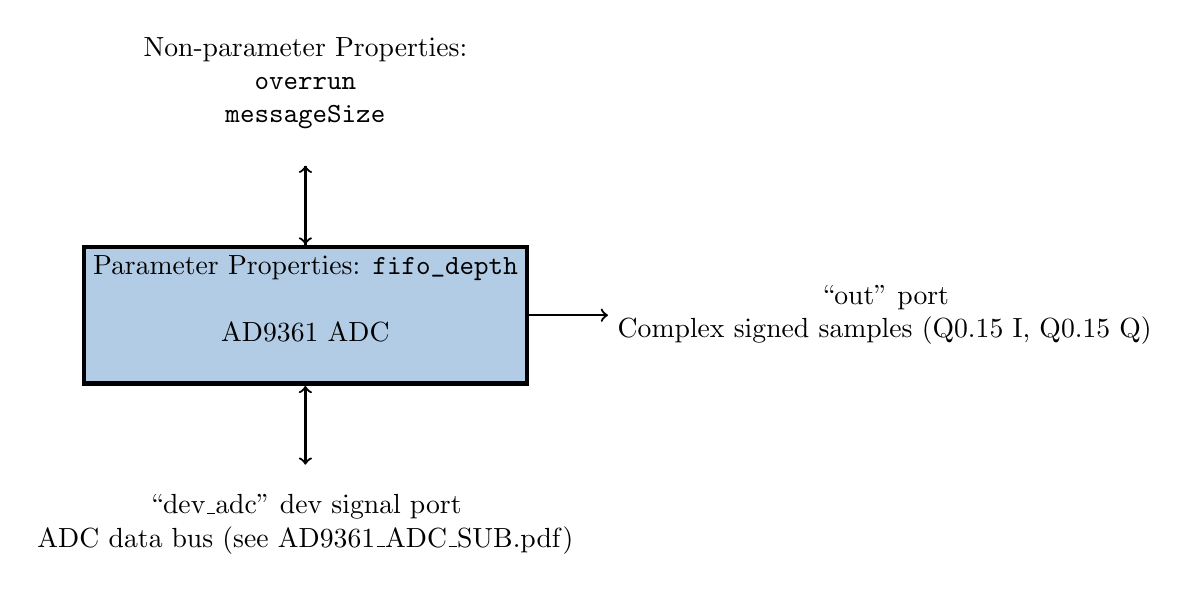
\begin{tikzpicture}[% List of styles applied to all, to override specify on a case-by-case
			every node/.style={
				align=center,  		% use this so that the "\\" for line break works
				minimum size=1.5cm	% creates space above and below text in rectangle
			},
			every edge/.style={draw,thick}
		]
		\node[rectangle,ultra thick,draw=black,fill=blue,minimum width=5 cm](R2){Parameter Properties: \verb+fifo_depth+ \\ \\ \Comp \\ };
		\node[rectangle,draw=white,fill=white](R3)[below= of R2]{``dev\_adc'' dev signal port\\ ADC data bus (see AD9361\_ADC\_SUB.pdf)};
		\node[rectangle,draw=white,fill=white](R4)[right= of R2]{``out'' port \\ Complex signed samples (Q0.15 I, Q0.15 Q)};
		\node[rectangle,draw=white,fill=white](R5)[above= of R2]{Non-parameter Properties:\\\verb+overrun+\\ \verb+messageSize+\\};
		\path[<->]
		(R3)edge []	node [] {} (R2);
		\path[->]
		(R2)edge []	node [] {} (R4)
		(R2)edge []	node [] {} (R5)
		(R5)edge []	node [] {} (R2)
		;
	\end{tikzpicture}
\end{center}
\section*{Source Dependencies}
\subsection*{\comp.hdl}
\begin{itemize}
	\item assets/hdl/devices/\comp.hdl/\comp.vhd
	\item core/hdl/primitives/util/adc\_fifo.vhd
	\item core/hdl/primitives/util/sync\_status.vhd
	\item core/hdl/primitives/util/util\_pkg.vhd
	\item core/hdl/primitives/bsv/imports/SyncFIFO.v
	\item core/hdl/primitives/bsv/imports/SyncResetA.v
	\item core/hdl/primitives/bsv/imports/SyncHandshake.v
	\item core/hdl/primitives/bsv/bsv\_pkg.vhd
\end{itemize}
\begin{landscape}

	\section*{Component Spec Properties}
	\begin{scriptsize}
		\begin{tabular}{|p{3.75cm}|p{1.25cm}|p{2cm}|p{2.75cm}|p{1.5cm}|p{1.5cm}|p{1cm}|p{5.25cm}|}
			\hline
			\rowcolor{blue}
			Name               & Type & SequenceLength & ArrayDimensions & Accessibility      & Valid Range & Default & Usage                                                                               \\
			\hline
			\verb+messageSize+ & Long & -              & -               & Initial, Readable  & Standard    & -       & Number of bytes in output message                                                   \\
			\hline
			\verb+overrun+     & Bool & -              & -               & Writable, Volatile & Standard    & -       & Flag set when ADC tries to load a sample and the ADC FIFO is full. Once high, this flag is not cleared (i.e. set low) until the property is written to again (the flag clears regardless of write value, i.e. writing true or false both result in a value of false, also note that a property write happens on reset).\\
			\hline
		\end{tabular}
	\end{scriptsize}

	\section*{Worker Properties}
	\subsection*{\comp.hdl}
	\begin{scriptsize}
		\begin{tabular}{|p{2cm}|p{2cm}|p{1cm}|p{2cm}|p{2cm}|p{2cm}|p{2cm}|p{1cm}|p{4.58cm}|}
			\hline
			\rowcolor{blue}
			Scope        & Name                 & Type & SequenceLength & ArrayDimensions & Accessibility & Valid Range        & Default & Usage                                                                                                                  \\
			\hline
			SpecProperty & \verb+messageSize+   & Long & -              & -               & Initial,Readable& Standard           & 8192    & Number of bytes in output message                                                                                      \\
			\hline
			SpecProperty & \verb+overrun+       & Bool & -              & -               & Writable,Volatile& Standard           & 0       & Flag set when ADC tries to load a sample and the ADC FIFO is full. Once high, this flag is not cleared (i.e. set low) until the property is written to again (the flag clears regardless of write value, i.e. writing true or false both result in a value of false, also note that a property write happens on reset).                                   \\
			\hline
			Property     & \verb+fifo_depth+    & ULong& -              & -               & Parameter     & Standard           & 0       & Depth in number of samples of the ADC-to-control clock domain crossing FIFO.                                   \\
			\hline
		\end{tabular}
	\end{scriptsize}

	\section*{Component Ports}
	\begin{scriptsize}
		\begin{tabular}{|p{2cm}|p{1.5cm}|p{4cm}|p{1.5cm}|p{1.5cm}|p{9.38cm}|}
			\hline
			\rowcolor{blue}
			Name & Producer & Protocol           & Optional & Advanced & Usage                  \\
			\hline
			out  & true     & iqstream\_protocol & true     & -        & Complex signed samples (Q0.15 I, Q0.15 Q). \\
			\hline
		\end{tabular}
	\end{scriptsize}
\pagebreak
	\section*{Worker Interfaces}
	\subsection*{\comp.hdl}
	\begin{scriptsize}
		\begin{tabular}{|p{2cm}|p{1.5cm}|p{1.5cm}|p{1.5cm}|p{13.8cm}|}
			\hline
			\rowcolor{blue}
			Type            & Name & DataWidth & Advanced & Usage                  \\
			\hline
			StreamInterface & out  & 32        & -        & Complex signed samples (Q0.15 I, Q0.15 Q). This port generates data and obeys backpressure. Because both backpressure from the \verb+out+ port and forward pressure from the \verb+dev_adc+ data bus exists, it is possible for samples to be dropped in the clock domain-crossing FIFO, i.e. seen on the \verb+dev_adc+ data bus but never make it to the output port. This event is monitored via the \verb+overrun+ property.  \\
			\hline
		\end{tabular}
	\end{scriptsize} \\ \\
	\begin{scriptsize}
		\begin{tabular}{|p{1.5cm}|p{1.4cm}|p{1.05cm}|p{1.25cm}|p{1.2cm}|p{3cm}|p{1.4cm}|p{0.9cm}|p{6.88cm}|}
			\hline
			\rowcolor{blue}
			Type                       & Name                            & Count & Optional & Master                & Signal                & Direction                  & Width                    & Description                                                                                                                  \\
			\hline
			\multirow{8}{*}{DevSignal} & \multirow{8}{*}{dev\_adc} & \multirow{8}{*}{1} & \multirow{8}{*}{False} & \multirow{8}{*}{True}  & present & Output&1& Value is 1 if a worker is connected to this devsignal port. \\
			\cline{6-9}
			&             &        &     &      & adc\_data\_I & Input     & 12     & Signed Q0.11 I value of ADC sample corresponding to RX channel 1. \\
			\cline{6-9}
			&             &        &     &      & adc\_data\_Q & Input     & 12     & Signed Q0.11 Q value of ADC sample corresponding to RX channel 1. \\
			\cline{6-9}
			&             &        &     &      & adc\_clk     & Input     & 1      & Clock for adc\_data\_I, adc\_data\_Q, and adc\_give. \\
			\cline{6-9}
			&             &        &     &      & adc\_give    & Input     & 1      & Indicates that the adc\_data\_I and adc\_data\_Q are valid and should be latched on the next rising edge of adc\_clk. \\
			\hline
		\end{tabular}
	\end{scriptsize}
\end{landscape}

\section*{Control Timing and Signals}
The \comp{}.hdl device worker contains two clock domains: the clock from the Control Plane, and the adc\_clk clock from the dev signal.\par\bigskip
\noindent The latency from the dev signal data bus to the output port is non-deterministic due to data flowing through an asynchronous FIFO with each side in a different clock domain. This non-determinism exists even in the absense of backpressure. In the presence of backpressure, the latency increases in an amount directly proportional to the degree to which the FIFO is full.

\section*{Worker Configuration Parameters}
\subsubsection*{\comp.hdl}
%\input{../../\ecomp.hdl/configurations.inc}
\section*{Performance and Resource Utilization}
\subsubsection*{\comp.hdl}
The FPGA resource utilization and Fmax are included for this worker. Fmax refers to the maximum allowable clock rate for any registered signal paths within a given clock domain for an FPGA design. Fmax in the table below is specific only to this worker and represents the maximum possible Fmax for any OpenCPI bitstream built with this worker included. Note that the Fmax value for a given clock domain for the final bitstream is often worse than the Fmax specific to this worker, even if this worker is the only one included in the bitstream. Note also that the DATA\_CLK\_P devsignal's rate will only ever go as high as 245.76 MHz\cite{adi_ug570}. \\ \\

%\input{../../\ecomp.hdl/utilization.inc}
\input{utilization_custom.inc}

\footnotetext[1]{\label{abc}These measurements were the result of a Vivado timing analysis which was different from the Vivado analysis performed by default for OpenCPI worker builds. For more info see Appendix \ref{appendix}}

\pagebreak
\section*{Test and Verification}
No unit test for this component exists. However, a hardware-in-the-loop
application (which is NOT a unit test) exists for testing purposes (see
assets/applications/ad9361\_adc\_test).

\begin{thebibliography}{1}

\bibitem{ad9361} AD9361 Datasheet and Product Info \\
\url{
https://www.analog.com/en/products/ad9361.html}
\bibitem{adi_ug570} AD9361 Reference Manual UG-570\\
AD9361\_Reference\_Manual\_UG-570.pdf
\bibitem{adc_sub_comp_datasheet} AD361 ADC Sub Component Data Sheet \\
\githubioURL{assets/AD9361_ADC_Sub.pdf}

\end{thebibliography}
\pagebreak
\section{Appendix 1 - AD9361 ADC Data Fidelity / Delay Setting Verification}
\subsection{FMCOMMS3 on ML605 FMC-LPC slot}
A custom script was run to report bit error rate vs. on-AD9361 RX data-clock delay settings. The following confirms both the ability of the ML605/FMCOMMS3 to have 100\% data fidelity up to the maximum data rate and the experimental range of valid delay settings. Each entry in the table below represents bit error rate in percent.
\lstset{language=bash, backgroundcolor=\color{lightgray}, columns=flexible, breaklines=true, prebreak=\textbackslash, basicstyle=\ttfamily, showstringspaces=false,upquote=true, aboveskip=\baselineskip, belowskip=\baselineskip}
\begin{lstlisting}[basicstyle=\scriptsize]
FIR enabled      : 0
Data port config : 1R1T
sample rate      : 2.083334e6 sps
 rx_data_clock_delay   rx_data_delay->
  |
  v
        0       1       2       3       4       5       6       7       8       9       10      11      12      13      14      15
0       11.1165 32.5526 38.0768 38.888  38.739  38.7141 38.7461 38.9165 error   38.7726 38.6963 38.887  38.8316 38.8514 38.8423 38.8295
1       0.175476
2       0
3       0
4       0
5       0
6       0
7       0
8       0
9       0
10      0
11      0
12      0
13      0
14      0
15      0
FIR enabled      : 0
Data port config : 1R1T
sample rate      : 25e6 sps
 rx_data_clock_delay   rx_data_delay->
  |
  v
        0       1       2       3       4       5       6       7       8       9       10      11      12      13      14      15
0       10.0082 32.0424 37.6495 38.6719 38.5193 38.267  38.6541 39.18   38.913  39.1368 38.7884 37.9674 37.9908 38.7934 38.827  37.885
1       0.0223796
2       0
3       0
4       0
5       0
6       0
7       0
8       0
9       0
10      0
11      0
12      0
13      0
14      0
15      0
FIR enabled      : 0
Data port config : 1R1T
sample rate      : 40e6 sps
 rx_data_clock_delay   rx_data_delay->
  |
  v
        0       1       2       3       4       5       6       7       8       9       10      11      12      13      14      15
0       10.0683 32.1218 37.4532 39.2014 39.1764 38.8275 37.9369 38.6688 38.5096 38.9964 38.5442 37.9761 38.4176 37.973  37.9934 38.9781
1       0.00101725
2       0
3       0
4       0
5       0
6       0
7       0
8       0
9       0
10      0
11      0
12      0
13      0
14      0
15      0
FIR enabled      : 0
Data port config : 1R1T
sample rate      : 61.44e6 sps
 rx_data_clock_delay   rx_data_delay->
  |
  v
        0       1       2       3       4       5       6       7       8       9       10      11      12      13      14      15
0       8.7087  31.222  36.0377 39.0559 38.7578 38.8687 38.5117 39.0518 38.8646 38.6719 38.3362 39.0422 38.4893 37.7355 39.0508 39.0106
1       0.161743
2       0
3       0
4       0
5       0
6       0
7       0
8       0
9       0
10      0
11      0
12      0
13      0
14      0
15      0
FIR enabled      : 0
Data port config : 2R2T
sample rate      : 2.083334e6 sps
 rx_data_clock_delay   rx_data_delay->
  |
  v
        0       1       2       3       4       5       6       7       8       9       10      11      12      13      14      15
0       error   31.9356 error   38.8067 38.7568 error   error   38.6948 38.6612 38.8941 38.6012 38.7405 38.7589 38.9399 38.7741 38.8087
1       0
2       0
3       0
4       0
5       0
6       0
7       0
8       0
9       0
10      0
11      0
12      0
13      0
14      0
15      error
FIR enabled      : 0
Data port config : 2R2T
sample rate      : 25e6 sps
 rx_data_clock_delay   rx_data_delay->
  |
  v
        0       1       2       3       4       5       6       7       8       9       10      11      12      13      14      15
0       10.2153 31.5826 37.1175 38.8011 38.7777 38.7955 38.9638 39.1596 38.6841 39.1734 38.7619 38.6576 38.6983 38.9506 38.5905 38.9964
1       0
2       0
3       0
4       0
5       0
6       0
7       0
8       0
9       0
10      0
11      0
12      0
13      0
14      0
15      0
FIR enabled      : 0
Data port config : 2R2T
sample rate      : 40e6 sps
 rx_data_clock_delay   rx_data_delay->
  |
  v
        0       1       2       3       4       5       6       7       8       9       10      11      12      13      14      15
0       19.9519 34.5505 38.4109 38.6759 38.8428 39.123  39.1123 38.7451 38.8947 37.7131 38.6642 38.6897 38.415  36.411  26.7649 11.1231
1       3.42967
2       0
3       0
4       0
5       0
6       0
7       0
8       0
9       0
10      0
11      0
12      3.35541
13      15.3783
14      34.4991
15      37.8092
FIR enabled      : 0
Data port config : 2R2T
sample rate      : 61.44e6 sps
 rx_data_clock_delay   rx_data_delay->
  |
  v
        0       1       2       3       4       5       6       7       8       9       10      11      12      13      14      15
0       9.56268 30.2144 37.0743 39.0889 38.6958 38.6719 39.1861 38.9008 37.7182 34.2031 20.5037 5.95449 0       0       0       0
1       0.54067
2       0
3       0
4       0
5       0
6       0.18158
7       7.34151
8       23.8927
9       36.7589
10      38.9262
11      39.0381
12      38.886
13      38.8255
14      39.1647
15      38.3784
\end{lstlisting}
\pagebreak
\section{Appendix 2 - Vivado Timing Analysis} \label{appendix}

The Vivado timing report that OpenCPI runs for device workers may erroneously report a max delay for a clocking path which should have been ignored. Custom Vivado tcl commands had to be run for this device worker to extract pertinent information from Vivado timing analysis. After building the worker, the following commands were run from the assets project directory (after the Vivado settings64.sh was sourced):
\begin{lstlisting}
cd hdl/devices/
vivado -mode tcl
\end{lstlisting}
Then the following commands were run inside the Vivado tcl terminal:
\begin{lstlisting}
open_project ad9361_adc.hdl/target-zynq/ad9361_adc_rv.xpr
synth_design -part xc7z020clg484-1 -top ad9361_adc_rv -mode out_of_context
create_clock -name clk1 -period 0.001 [get_nets {ctl_in[Clk]}]
create_clock -name clk2 -period 0.001 [get_nets {dev_adc_in[adc_clk]}]
set_clock_groups -asynchronous -group [get_clocks clk1] -group [get_clocks clk2]
report_timing -delay_type min_max -sort_by slack -input_pins -group clk1
report_timing -delay_type min_max -sort_by slack -input_pins -group clk2
\end{lstlisting}
The following is the output of the timing reports. The Fmax for the control plane clock for this worker is computed as the maximum magnitude slack with a control plane clock of 1 ps plus 2 times the assumed 1 ps control plane clock period (4.933 ns + 0.002 ns = 4.935 ns, 1/4.935 ns = 202.63 MHz). The Fmax for the adc\_clk clock from the devsignal is computed as the maximum magnitude slack with adc\_clk of 1 ps plus 2 times the assumed 1 ps adc\_clk period (2.947 ns + 0.002 ns = 2.949 ns, 1/2.949 ns = 339.10 MHz).
\fontsize{6}{12}\selectfont
\begin{lstlisting}
Vivado% report_timing -delay_type min_max -sort_by slack -input_pins -group clk1

Timing Report

Slack (VIOLATED) :        -4.933ns  (required time - arrival time)
  Source:                 wci/messageSize_property/value_reg[7]/C
                            (rising edge-triggered cell FDRE clocked by clk1  {rise@0.000ns fall@0.001ns period=0.001ns})
  Destination:            worker/fifo/samplesInMessage_r_reg[0]/S
                            (rising edge-triggered cell FDSE clocked by clk1  {rise@0.000ns fall@0.001ns period=0.001ns})
  Path Group:             clk1
  Path Type:              Setup (Max at Slow Process Corner)
  Requirement:            0.002ns  (clk1 rise@0.002ns - clk1 rise@0.000ns)
  Data Path Delay:        4.327ns  (logic 2.025ns (46.799%)  route 2.302ns (53.201%))
  Logic Levels:           5  (CARRY4=3 LUT5=1 LUT6=1)
  Clock Path Skew:        -0.049ns (DCD - SCD + CPR)
    Destination Clock Delay (DCD):    0.924ns = ( 0.926 - 0.002 )
    Source Clock Delay      (SCD):    0.973ns
    Clock Pessimism Removal (CPR):    0.000ns
  Clock Uncertainty:      0.035ns  ((TSJ^2 + TIJ^2)^1/2 + DJ) / 2 + PE
    Total System Jitter     (TSJ):    0.071ns
    Total Input Jitter      (TIJ):    0.000ns
    Discrete Jitter          (DJ):    0.000ns
    Phase Error              (PE):    0.000ns

    Location             Delay type                Incr(ns)  Path(ns)    Netlist Resource(s)
  -------------------------------------------------------------------    -------------------
                         (clock clk1 rise edge)       0.000     0.000 r
                                                      0.000     0.000 r  ctl_in[Clk] (IN)
                         net (fo=155, unset)          0.973     0.973    wci/messageSize_property/ctl_in[Clk]
                         FDRE                                         r  wci/messageSize_property/value_reg[7]/C
  -------------------------------------------------------------------    -------------------
                         FDRE (Prop_fdre_C_Q)         0.518     1.491 r  wci/messageSize_property/value_reg[7]/Q
                         net (fo=2, unplaced)         0.976     2.467    wci/messageSize_property/Q[6]
                                                                      r  wci/messageSize_property/b_carry_i_3/I0
                         LUT6 (Prop_lut6_I0_O)        0.295     2.762 r  wci/messageSize_property/b_carry_i_3/O
                         net (fo=1, unplaced)         0.000     2.762    worker/fifo/S[1]
                                                                      r  worker/fifo/b_carry/S[1]
                         CARRY4 (Prop_carry4_S[1]_CO[3])
                                                      0.533     3.295 r  worker/fifo/b_carry/CO[3]
                         net (fo=1, unplaced)         0.009     3.304    worker/fifo/b_carry_n_0
                                                                      r  worker/fifo/b_carry__0/CI
                         CARRY4 (Prop_carry4_CI_CO[3])
                                                      0.117     3.421 r  worker/fifo/b_carry__0/CO[3]
                         net (fo=1, unplaced)         0.000     3.421    worker/fifo/b_carry__0_n_0
                                                                      r  worker/fifo/b_carry__1/CI
                         CARRY4 (Prop_carry4_CI_CO[2])
                                                      0.252     3.673 r  worker/fifo/b_carry__1/CO[2]
                         net (fo=3, unplaced)         0.470     4.143    wci/wci_decode/CO[0]
                                                                      r  wci/wci_decode/samplesInMessage_r[0]_i_1/I3
                         LUT5 (Prop_lut5_I3_O)        0.310     4.453 r  wci/wci_decode/samplesInMessage_r[0]_i_1/O
                         net (fo=32, unplaced)        0.847     5.300    worker/fifo/or
                         FDSE                                         r  worker/fifo/samplesInMessage_r_reg[0]/S
  -------------------------------------------------------------------    -------------------

                         (clock clk1 rise edge)       0.002     0.002 r
                                                      0.000     0.002 r  ctl_in[Clk] (IN)
                         net (fo=155, unset)          0.924     0.926    worker/fifo/ctl_in[Clk]
                         FDSE                                         r  worker/fifo/samplesInMessage_r_reg[0]/C
                         clock pessimism              0.000     0.926
                         clock uncertainty           -0.035     0.891
                         FDSE (Setup_fdse_C_S)       -0.524     0.367    worker/fifo/samplesInMessage_r_reg[0]
  -------------------------------------------------------------------
                         required time                          0.367
                         arrival time                          -5.300
  -------------------------------------------------------------------
                         slack                                 -4.933

Vivado% report_timing -delay_type min_max -sort_by slack -input_pins -group clk2

Timing Report

Slack (VIOLATED) :        -2.947ns  (required time - arrival time)
  Source:                 worker/fifo/fifo/sGEnqPtr_reg[1]/C
                            (rising edge-triggered cell FDCE clocked by clk2  {rise@0.000ns fall@0.001ns period=0.001ns})
  Destination:            worker/fifo/fifo/sNotFullReg_reg/D
                            (rising edge-triggered cell FDCE clocked by clk2  {rise@0.000ns fall@0.001ns period=0.001ns})
  Path Group:             clk2
  Path Type:              Setup (Max at Slow Process Corner)
  Requirement:            0.002ns  (clk2 rise@0.002ns - clk2 rise@0.000ns)
  Data Path Delay:        2.942ns  (logic 1.061ns (36.064%)  route 1.881ns (63.936%))
  Logic Levels:           3  (LUT4=1 LUT6=2)
  Clock Path Skew:        -0.049ns (DCD - SCD + CPR)
    Destination Clock Delay (DCD):    0.924ns = ( 0.926 - 0.002 )
    Source Clock Delay      (SCD):    0.973ns
    Clock Pessimism Removal (CPR):    0.000ns
  Clock Uncertainty:      0.035ns  ((TSJ^2 + TIJ^2)^1/2 + DJ) / 2 + PE
    Total System Jitter     (TSJ):    0.071ns
    Total Input Jitter      (TIJ):    0.000ns
    Discrete Jitter          (DJ):    0.000ns
    Phase Error              (PE):    0.000ns

    Location             Delay type                Incr(ns)  Path(ns)    Netlist Resource(s)
  -------------------------------------------------------------------    -------------------
                         (clock clk2 rise edge)       0.000     0.000 r
                                                      0.000     0.000 r  dev_adc_in[adc_clk] (IN)
                         net (fo=33, unset)           0.973     0.973    worker/fifo/fifo/dev_adc_in[adc_clk]
                         FDCE                                         r  worker/fifo/fifo/sGEnqPtr_reg[1]/C
  -------------------------------------------------------------------    -------------------
                         FDCE (Prop_fdce_C_Q)         0.518     1.491 r  worker/fifo/fifo/sGEnqPtr_reg[1]/Q
                         net (fo=3, unplaced)         0.983     2.474    worker/fifo/fifo/p_0_in[0]
                                                                      r  worker/fifo/fifo/sNotFullReg_i_6/I0
                         LUT6 (Prop_lut6_I0_O)        0.295     2.769 r  worker/fifo/fifo/sNotFullReg_i_6/O
                         net (fo=1, unplaced)         0.449     3.218    worker/fifo/fifo/sNotFullReg_i_6_n_0
                                                                      r  worker/fifo/fifo/sNotFullReg_i_4/I3
                         LUT4 (Prop_lut4_I3_O)        0.124     3.342 r  worker/fifo/fifo/sNotFullReg_i_4/O
                         net (fo=1, unplaced)         0.449     3.791    worker/fifo/fifo/sNextNotFull__12
                                                                      r  worker/fifo/fifo/sNotFullReg_i_1/I5
                         LUT6 (Prop_lut6_I5_O)        0.124     3.915 r  worker/fifo/fifo/sNotFullReg_i_1/O
                         net (fo=1, unplaced)         0.000     3.915    worker/fifo/fifo/sNotFullReg_i_1_n_0
                         FDCE                                         r  worker/fifo/fifo/sNotFullReg_reg/D
  -------------------------------------------------------------------    -------------------

                         (clock clk2 rise edge)       0.002     0.002 r
                                                      0.000     0.002 r  dev_adc_in[adc_clk] (IN)
                         net (fo=33, unset)           0.924     0.926    worker/fifo/fifo/dev_adc_in[adc_clk]
                         FDCE                                         r  worker/fifo/fifo/sNotFullReg_reg/C
                         clock pessimism              0.000     0.926
                         clock uncertainty           -0.035     0.891
                         FDCE (Setup_fdce_C_D)        0.077     0.968    worker/fifo/fifo/sNotFullReg_reg
  -------------------------------------------------------------------
                         required time                          0.968
                         arrival time                          -3.915
  -------------------------------------------------------------------
                         slack                                 -2.947


\end{lstlisting}
\fontsize{10}{12}\selectfont
These calculations can be verified by replacing the \texttt{create\_clock} lines above with the following values and rerunning the \texttt{report\_timing} commands and observing a value of 0.000 ns for the slacks:
\begin{lstlisting}
create_clock -name clk1 -period 4.935 [get_nets {ctl_in[Clk]}]
create_clock -name clk2 -period 2.949 [get_nets {dev_adc_in[adc_clk]}]
report_timing -delay_type min_max -sort_by slack -input_pins -group clk1
report_timing -delay_type min_max -sort_by slack -input_pins -group clk2
\end{lstlisting}
\fontsize{6}{12}\selectfont
\begin{lstlisting}
Vivado% report_timing -delay_type min_max -sort_by slack -input_pins -group clk1

Timing Report

Slack (MET) :             0.000ns  (required time - arrival time)
  Source:                 wci/messageSize_property/value_reg[7]/C
                            (rising edge-triggered cell FDRE clocked by clk1  {rise@0.000ns fall@2.467ns period=4.935ns})
  Destination:            worker/fifo/samplesInMessage_r_reg[0]/S
                            (rising edge-triggered cell FDSE clocked by clk1  {rise@0.000ns fall@2.467ns period=4.935ns})
  Path Group:             clk1
  Path Type:              Setup (Max at Slow Process Corner)
  Requirement:            4.935ns  (clk1 rise@4.935ns - clk1 rise@0.000ns)
  Data Path Delay:        4.327ns  (logic 2.025ns (46.799%)  route 2.302ns (53.201%))
  Logic Levels:           5  (CARRY4=3 LUT5=1 LUT6=1)
  Clock Path Skew:        -0.049ns (DCD - SCD + CPR)
    Destination Clock Delay (DCD):    0.924ns = ( 5.859 - 4.935 )
    Source Clock Delay      (SCD):    0.973ns
    Clock Pessimism Removal (CPR):    0.000ns
  Clock Uncertainty:      0.035ns  ((TSJ^2 + TIJ^2)^1/2 + DJ) / 2 + PE
    Total System Jitter     (TSJ):    0.071ns
    Total Input Jitter      (TIJ):    0.000ns
    Discrete Jitter          (DJ):    0.000ns
    Phase Error              (PE):    0.000ns

    Location             Delay type                Incr(ns)  Path(ns)    Netlist Resource(s)
  -------------------------------------------------------------------    -------------------
                         (clock clk1 rise edge)       0.000     0.000 r
                                                      0.000     0.000 r  ctl_in[Clk] (IN)
                         net (fo=155, unset)          0.973     0.973    wci/messageSize_property/ctl_in[Clk]
                         FDRE                                         r  wci/messageSize_property/value_reg[7]/C
  -------------------------------------------------------------------    -------------------
                         FDRE (Prop_fdre_C_Q)         0.518     1.491 r  wci/messageSize_property/value_reg[7]/Q
                         net (fo=2, unplaced)         0.976     2.467    wci/messageSize_property/Q[6]
                                                                      r  wci/messageSize_property/b_carry_i_3/I0
                         LUT6 (Prop_lut6_I0_O)        0.295     2.762 r  wci/messageSize_property/b_carry_i_3/O
                         net (fo=1, unplaced)         0.000     2.762    worker/fifo/S[1]
                                                                      r  worker/fifo/b_carry/S[1]
                         CARRY4 (Prop_carry4_S[1]_CO[3])
                                                      0.533     3.295 r  worker/fifo/b_carry/CO[3]
                         net (fo=1, unplaced)         0.009     3.304    worker/fifo/b_carry_n_0
                                                                      r  worker/fifo/b_carry__0/CI
                         CARRY4 (Prop_carry4_CI_CO[3])
                                                      0.117     3.421 r  worker/fifo/b_carry__0/CO[3]
                         net (fo=1, unplaced)         0.000     3.421    worker/fifo/b_carry__0_n_0
                                                                      r  worker/fifo/b_carry__1/CI
                         CARRY4 (Prop_carry4_CI_CO[2])
                                                      0.252     3.673 r  worker/fifo/b_carry__1/CO[2]
                         net (fo=3, unplaced)         0.470     4.143    wci/wci_decode/CO[0]
                                                                      r  wci/wci_decode/samplesInMessage_r[0]_i_1/I3
                         LUT5 (Prop_lut5_I3_O)        0.310     4.453 r  wci/wci_decode/samplesInMessage_r[0]_i_1/O
                         net (fo=32, unplaced)        0.847     5.300    worker/fifo/or
                         FDSE                                         r  worker/fifo/samplesInMessage_r_reg[0]/S
  -------------------------------------------------------------------    -------------------

                         (clock clk1 rise edge)       4.935     4.935 r
                                                      0.000     4.935 r  ctl_in[Clk] (IN)
                         net (fo=155, unset)          0.924     5.859    worker/fifo/ctl_in[Clk]
                         FDSE                                         r  worker/fifo/samplesInMessage_r_reg[0]/C
                         clock pessimism              0.000     5.859
                         clock uncertainty           -0.035     5.824
                         FDSE (Setup_fdse_C_S)       -0.524     5.300    worker/fifo/samplesInMessage_r_reg[0]
  -------------------------------------------------------------------
                         required time                          5.300
                         arrival time                          -5.300
  -------------------------------------------------------------------
                         slack                                  0.000




Vivado% report_timing -delay_type min_max -sort_by slack -input_pins -group clk2

Timing Report

Slack (MET) :             0.000ns  (required time - arrival time)
  Source:                 worker/fifo/fifo/sGEnqPtr_reg[1]/C
                            (rising edge-triggered cell FDCE clocked by clk2  {rise@0.000ns fall@1.474ns period=2.949ns})
  Destination:            worker/fifo/fifo/sNotFullReg_reg/D
                            (rising edge-triggered cell FDCE clocked by clk2  {rise@0.000ns fall@1.474ns period=2.949ns})
  Path Group:             clk2
  Path Type:              Setup (Max at Slow Process Corner)
  Requirement:            2.949ns  (clk2 rise@2.949ns - clk2 rise@0.000ns)
  Data Path Delay:        2.942ns  (logic 1.061ns (36.064%)  route 1.881ns (63.936%))
  Logic Levels:           3  (LUT4=1 LUT6=2)
  Clock Path Skew:        -0.049ns (DCD - SCD + CPR)
    Destination Clock Delay (DCD):    0.924ns = ( 3.873 - 2.949 )
    Source Clock Delay      (SCD):    0.973ns
    Clock Pessimism Removal (CPR):    0.000ns
  Clock Uncertainty:      0.035ns  ((TSJ^2 + TIJ^2)^1/2 + DJ) / 2 + PE
    Total System Jitter     (TSJ):    0.071ns
    Total Input Jitter      (TIJ):    0.000ns
    Discrete Jitter          (DJ):    0.000ns
    Phase Error              (PE):    0.000ns

    Location             Delay type                Incr(ns)  Path(ns)    Netlist Resource(s)
  -------------------------------------------------------------------    -------------------
                         (clock clk2 rise edge)       0.000     0.000 r
                                                      0.000     0.000 r  dev_adc_in[adc_clk] (IN)
                         net (fo=33, unset)           0.973     0.973    worker/fifo/fifo/dev_adc_in[adc_clk]
                         FDCE                                         r  worker/fifo/fifo/sGEnqPtr_reg[1]/C
  -------------------------------------------------------------------    -------------------
                         FDCE (Prop_fdce_C_Q)         0.518     1.491 r  worker/fifo/fifo/sGEnqPtr_reg[1]/Q
                         net (fo=3, unplaced)         0.983     2.474    worker/fifo/fifo/p_0_in[0]
                                                                      r  worker/fifo/fifo/sNotFullReg_i_6/I0
                         LUT6 (Prop_lut6_I0_O)        0.295     2.769 r  worker/fifo/fifo/sNotFullReg_i_6/O
                         net (fo=1, unplaced)         0.449     3.218    worker/fifo/fifo/sNotFullReg_i_6_n_0
                                                                      r  worker/fifo/fifo/sNotFullReg_i_4/I3
                         LUT4 (Prop_lut4_I3_O)        0.124     3.342 r  worker/fifo/fifo/sNotFullReg_i_4/O
                         net (fo=1, unplaced)         0.449     3.791    worker/fifo/fifo/sNextNotFull__12
                                                                      r  worker/fifo/fifo/sNotFullReg_i_1/I5
                         LUT6 (Prop_lut6_I5_O)        0.124     3.915 r  worker/fifo/fifo/sNotFullReg_i_1/O
                         net (fo=1, unplaced)         0.000     3.915    worker/fifo/fifo/sNotFullReg_i_1_n_0
                         FDCE                                         r  worker/fifo/fifo/sNotFullReg_reg/D
  -------------------------------------------------------------------    -------------------

                         (clock clk2 rise edge)       2.949     2.949 r
                                                      0.000     2.949 r  dev_adc_in[adc_clk] (IN)
                         net (fo=33, unset)           0.924     3.873    worker/fifo/fifo/dev_adc_in[adc_clk]
                         FDCE                                         r  worker/fifo/fifo/sNotFullReg_reg/C
                         clock pessimism              0.000     3.873
                         clock uncertainty           -0.035     3.838
                         FDCE (Setup_fdce_C_D)        0.077     3.915    worker/fifo/fifo/sNotFullReg_reg
  -------------------------------------------------------------------
                         required time                          3.915
                         arrival time                          -3.915
  -------------------------------------------------------------------
                         slack                                  0.000





\end{lstlisting}

\fontsize{6}{12}\selectfont
\end{document}
